\chapter{Training our own models.}

\section{Data sets}
In the following we will use two different datasets. 1) \emph{Caltech} \footnote{Available at \footnote{http://www.vision.caltech.edu/html-files/archive.html}} which consists of "450 frontal face images of 27 or so unique people." and 2) \emph{FFHQ}\footnote{Available at \footnote{https://github.com/NVlabs/ffhq-dataset}} Here we use the 5000 of the provided thumbnails of resolution 128x128.


The FFHQ dataset is already preprocessed such that the faces are aligned and the images are of the same dimensions. For Caltech however we need to do this preprocessing manually.

In the Github repository for this project we provide code to download both datasets with additional preprocessing of the Caltech dataset.

% We use OpenCVs implementation of the haarcascade to make bounding boxes around the

In Figure \ref{rawdata} we see a random sample of the processed images from the Caltech \ref{raw-caltech} and FFHQ \ref{raw-ffhq} datasets respectively.

\begin{figure}[h!]
    \centering
    \begin{subfigure}[b]{0.45\textwidth}
        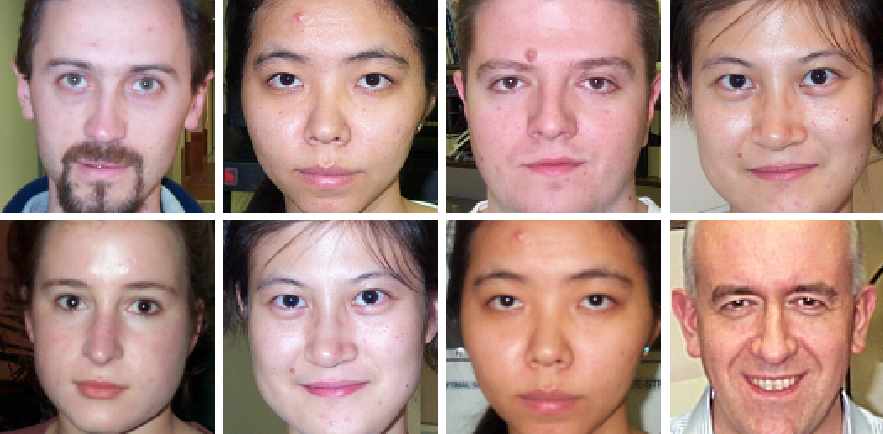
\includegraphics[width=\textwidth]{fig/data/caltech}
        \caption{Caltech dataset}
        \label{raw-caltech}
    \end{subfigure}
    ~
    \begin{subfigure}[b]{0.45\textwidth}
        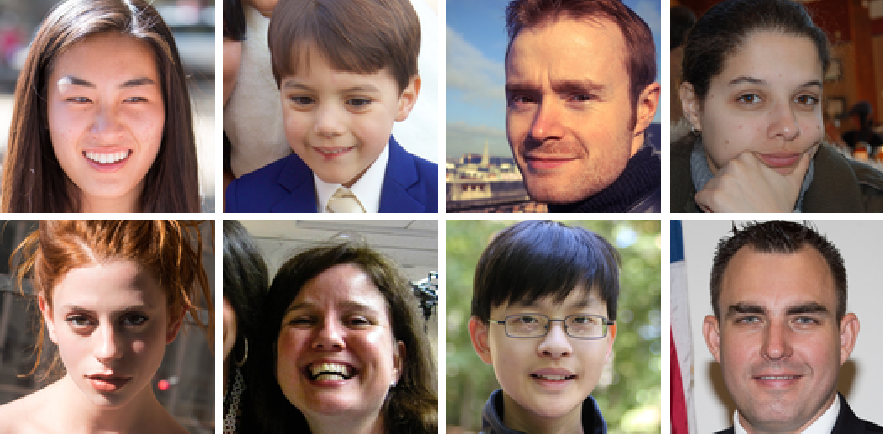
\includegraphics[width=\textwidth]{fig/data/ffhq}
        \caption{FFHQ dataset}
        \label{raw-ffhq}
    \end{subfigure}

    \caption{The raw data from the Caltech and FFHQ datasets respectively. This figure is the only one containing images of real people in the report.}
    \label{rawdata}
\end{figure}


\section{Principal Component Analysis }
In this section we explore the results of using Principal Component Analysis (PCA) for face synthesis. PCA is predominately used for dimensionality reduction but here we will use it for synthesis.

The goal of PCA is to find the Principal Components which are the directions of greatest variance in the dataset. These directions are the eigenvectors or, in this context, eigenfaces of the covariance matrix.

Let $\tilde{\mathbf{X}} = \mathbf{X} - \bar{\mathbf{X}}$ then $\mathbf{X}^T\mathbf{X}$ is the covariance matrix we find the eigenfaces the usual way by demanding that $\det(\mathbf{X}^T\mathbf{X} - \lambda) = 0$
We then sort the eigenface after eigenvalue $\lambda$ in order of descending variance. In Figure \ref{eigenface} we see the first 8 eigenfaces.

\begin{figure}
  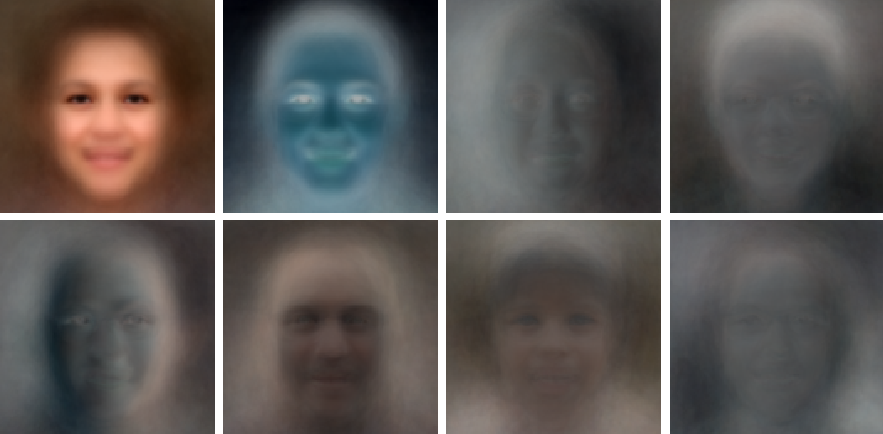
\includegraphics[width=\textwidth]{fig/PCA/pca}
  \caption{Eigenfaces of the FFHQ dataset.}
  \label{eigenface}
\end{figure}

We can generate new synthetic faces $F$ by adding a linear combination of the
eigenfaces $F_i$ to the mean face $F_m$.

\begin{align}
F  = F_m + \sum_{i} \alpha_i F_i
\end{align}
in Figure \ref{pca-components} we see the results of varying the first six
principal components.

In order it seems that the Principal Component control aspects of 1) and 2) Color 3) direction of lighting 4) age 5) pose and 6) gender.



\section{DCGAN}







% \begin{figure}
%     \centering
%     \begin{subfigure}[b]{0.3\textwidth}
%         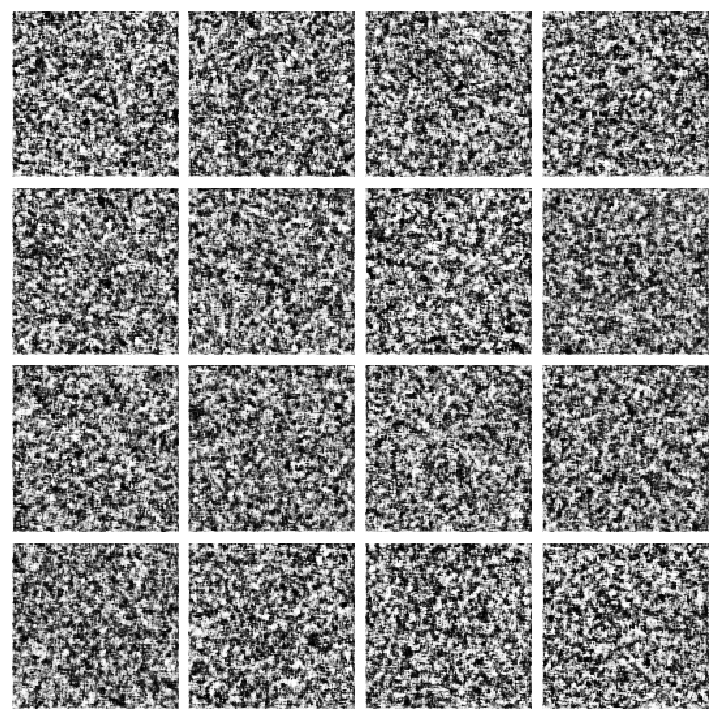
\includegraphics[width=\textwidth]{fig/dcgan/epoch0}
%         \caption{Epoch 0}
%     \end{subfigure}
%     ~
%     \begin{subfigure}[b]{0.3\textwidth}
%         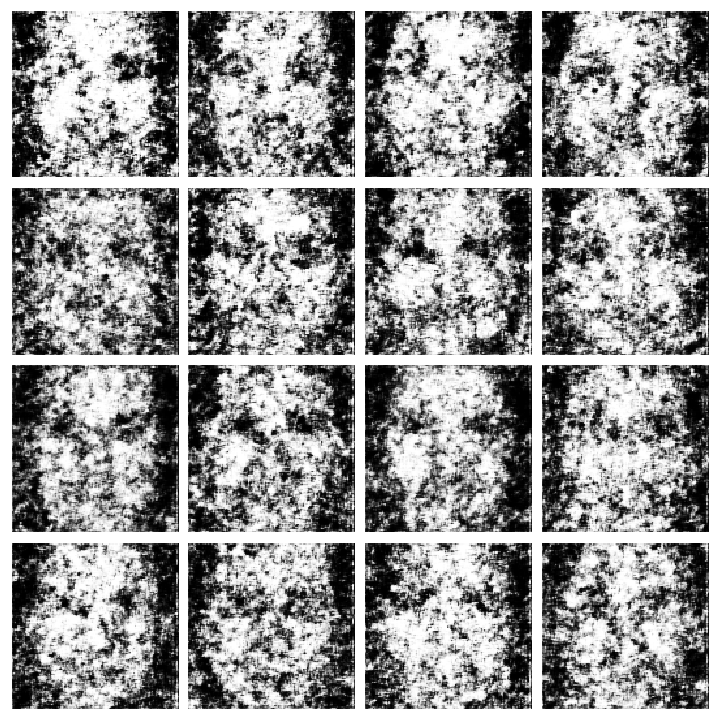
\includegraphics[width=\textwidth]{fig/dcgan/epoch10}
%         \caption{Epoch 10}
%     \end{subfigure}
%     ~
%     \begin{subfigure}[b]{0.3\textwidth}
%         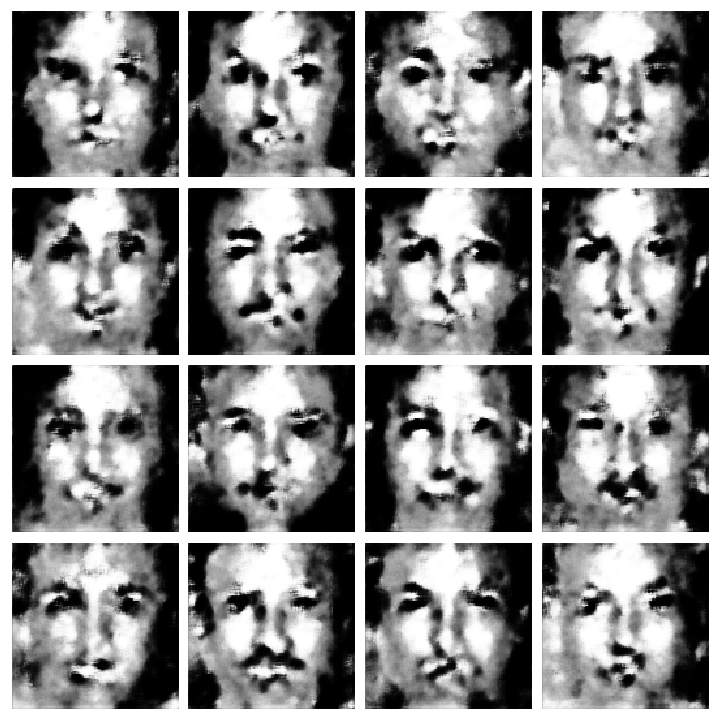
\includegraphics[width=\textwidth]{fig/dcgan/epoch100}
%         \caption{Epoch 100}
%     \end{subfigure}
%
%     \begin{subfigure}[b]{0.3\textwidth}
%         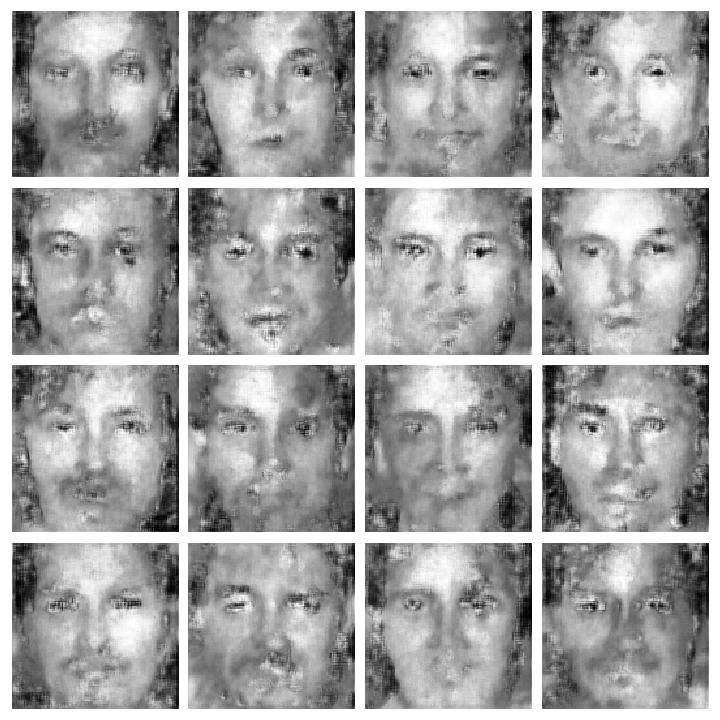
\includegraphics[width=\textwidth]{fig/dcgan/epoch200}
%         \caption{Epoch 200}
%     \end{subfigure}
%     ~
%     \begin{subfigure}[b]{0.3\textwidth}
%         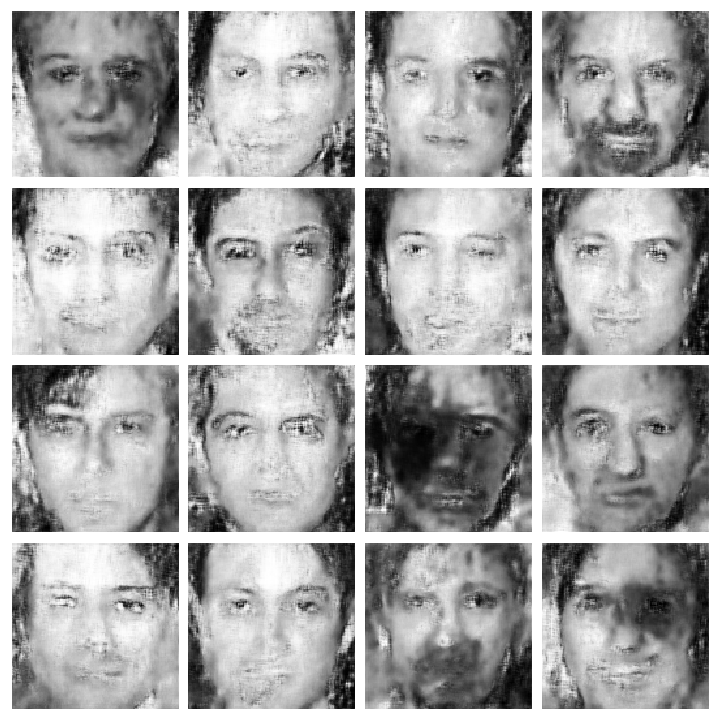
\includegraphics[width=\textwidth]{fig/dcgan/epoch400}
%         \caption{Epoch 400}
%     \end{subfigure}
%     ~
%     \begin{subfigure}[b]{0.3\textwidth}
%         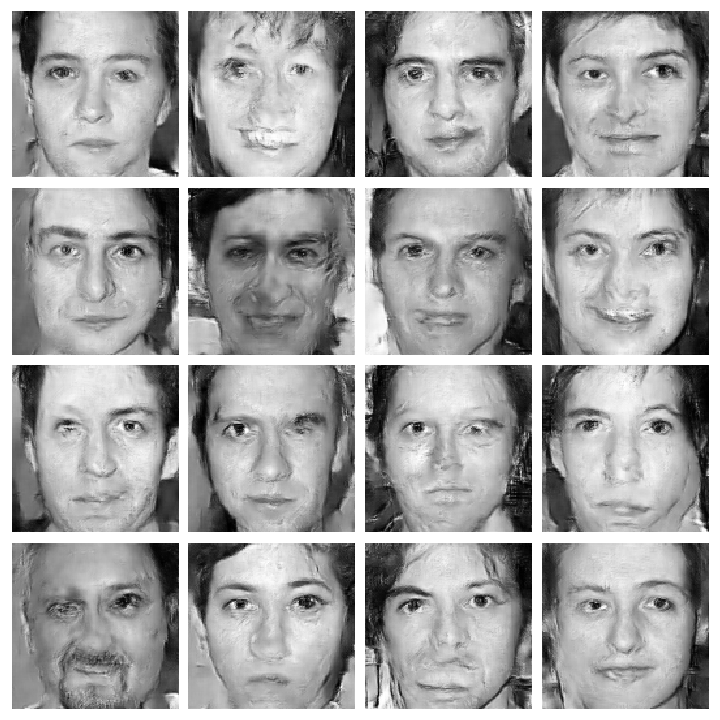
\includegraphics[width=\textwidth]{fig/dcgan/epoch4000}
%         \caption{Epoch 4000}
%     \end{subfigure}
%
%     \caption{Samples from DCGAN during traning on the Caltech dataset}
% \end{figure}
